\chapter{Introduction}
This documentation contains information about the specifications, design, architecture and functionality of the electrically propulsed car dubbed 'AU2'. This system has been designed to be able to compete in Shell Eco Marathon (in the Prototype - Battery-electric category).

\begin{figure}[H]
	\centering
	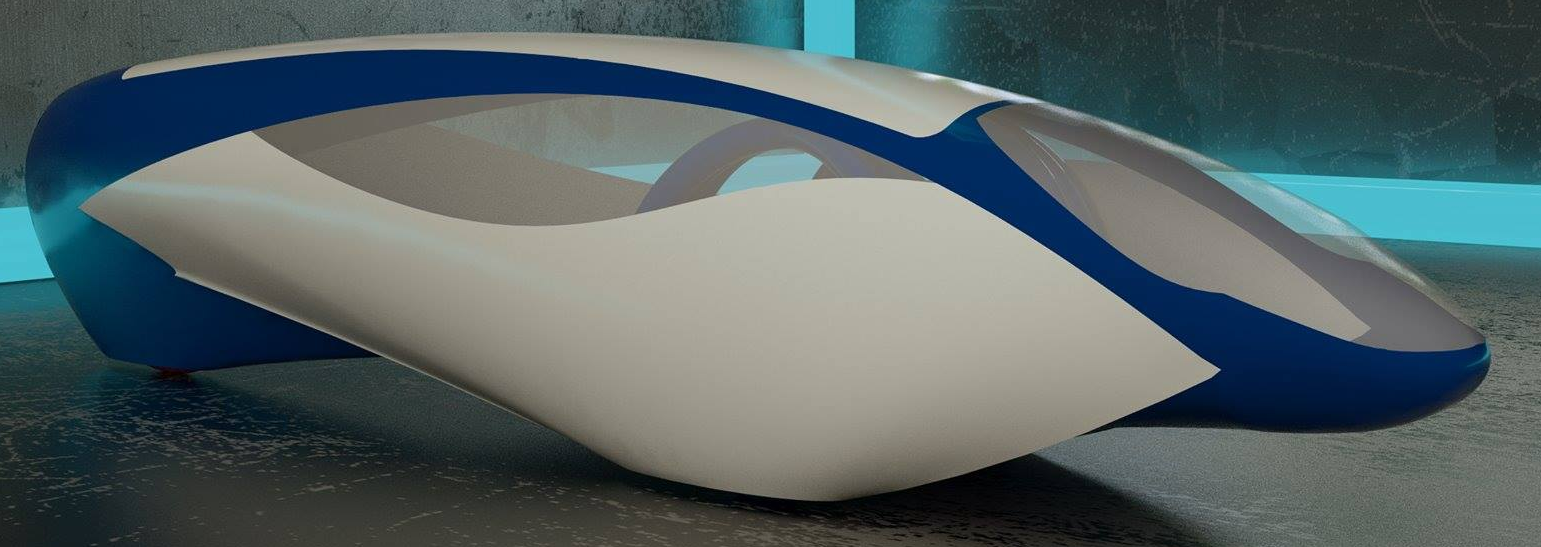
\includegraphics[width=0.6\linewidth]{Introduction/Model}
	\caption{Computer generated model of AU2}
	\label{fig:System_model}
\end{figure}

\section{System description}

The primary purpose of the car is to be as energy-effecient as possible, as this is the goal of Shell Eco Marathon. This is done by letting the car use a driving-technique called 'coast-and-burn'. This technique is explained in greater details in later chapters, but the basic principle is to let the car coast without propulsion for as long as possible and thereby minimizing the energy-consumption. This coast-and-burn technique can be turned on or off by the car's driver.

In order for the car to follow the technique's procedures correctly it has a variable energy-output to the electric motor. Furthermore, the car constantly measures the current speed and the amount of energy consumed. The measured parameters from a test-drive can be collected on a SD-card, if the user inserts such a card in the built-in SD-socket.

The car uses rechargable LiPo batteries which can be easily be inserted/removed to allow a mostly continuous driving experience. The battery is under constant surveillance by a Battery Management System (BMS) which measures the battery's energy-output and current temperature. This subsystem serves to protects the battery from overheating and protects the other circuits from an over-current.

As the car is designed to compete in Shell Eco-Marathon it must follow the safety procedures set down by Shell. This means that the car has a built-in safety mechanism. This machanism consists of two switches: an on/off-switch and a dead mans's switch. The dead man's switch must be pressed by the driver at all times in order for the car to drive.
Lastly, the car contains an electrical horn which can be activated by the driver.

\section{List of terms}
The following list explains the various terms which have been used to refer to certain parts or subsystems in this documentation.

\begin{itemize}
	\item \textbf{SEM}\\
	Refers to Shell Eco Marathon which the car is designed to compete in.
	\item \textbf{Coast-and-burn}\\
	Refers to the driving algorithm which the car follows.
	\item \textbf{BMS}\\
	Refers to the Battery Management System which manages the output from the rechargable battery in order to protect the battery, as well as the other electrical systems in the car.
\end{itemize}